\documentclass[10pt,a4paper]{article}
\usepackage[utf8]{inputenc}
\usepackage[german]{babel}
\usepackage{amsmath}
\usepackage{amsfonts}
\usepackage{amssymb}
\usepackage{graphicx}
\usepackage[left=2cm,right=2cm,top=2cm,bottom=2cm]{geometry}

\begin{document}

\section*{Aufgabe 11.1}

Wie liest man die KMF aus einem KV-Diagramm ab?
Wie baut man einen Tristate-Puffer?

\section*{Aufgabe 11.2}

\begin{tabular}{c|c|c|c}
a & b & $\overline{ab}$ & $\overline{a} + \overline{b}$\\
\hline
0 & 0 & 1 & 1\\
\hline
0 & 1 & 1 & 1\\
\hline
1 & 0 & 1 & 1\\
\hline
1 & 1 & 0 & 0
\end{tabular}
\\
\begin{tabular}{c|c|c|c}
a & b & $\overline{a + b}$ & $\overline{a}\overline{b}$\\
\hline
0 & 0 & 1 & 1\\
\hline
0 & 1 & 0 & 0\\
\hline
1 & 0 & 0 & 0\\
\hline
1 & 1 & 0 & 0
\end{tabular}

\begin{align*}
\overline{ab} & = \overline{ab1} = \overline{ab((\overline{a} + \overline{b}) + \overline{(\overline{a} + \overline{b})})} = \overline{(ab(\overline{a} + \overline{b})) + (ab\overline{(\overline{a} + \overline{b})})} = \overline{(ab\overline{a} + ab\overline{b}) + (ab\overline{(\overline{a} + \overline{b})})} = \overline{(a\overline{a}b + ab\overline{b}) + (ab\overline{(\overline{a} + \overline{b})})}\\
& = \overline{(0 + 0) + (ab\overline{(\overline{a} + \overline{b})})} = \overline{ab\overline{(\overline{a} + \overline{b})}}\\
\end{align*}

\section*{Aufgabe 11.3}

\begin{figure}[h]
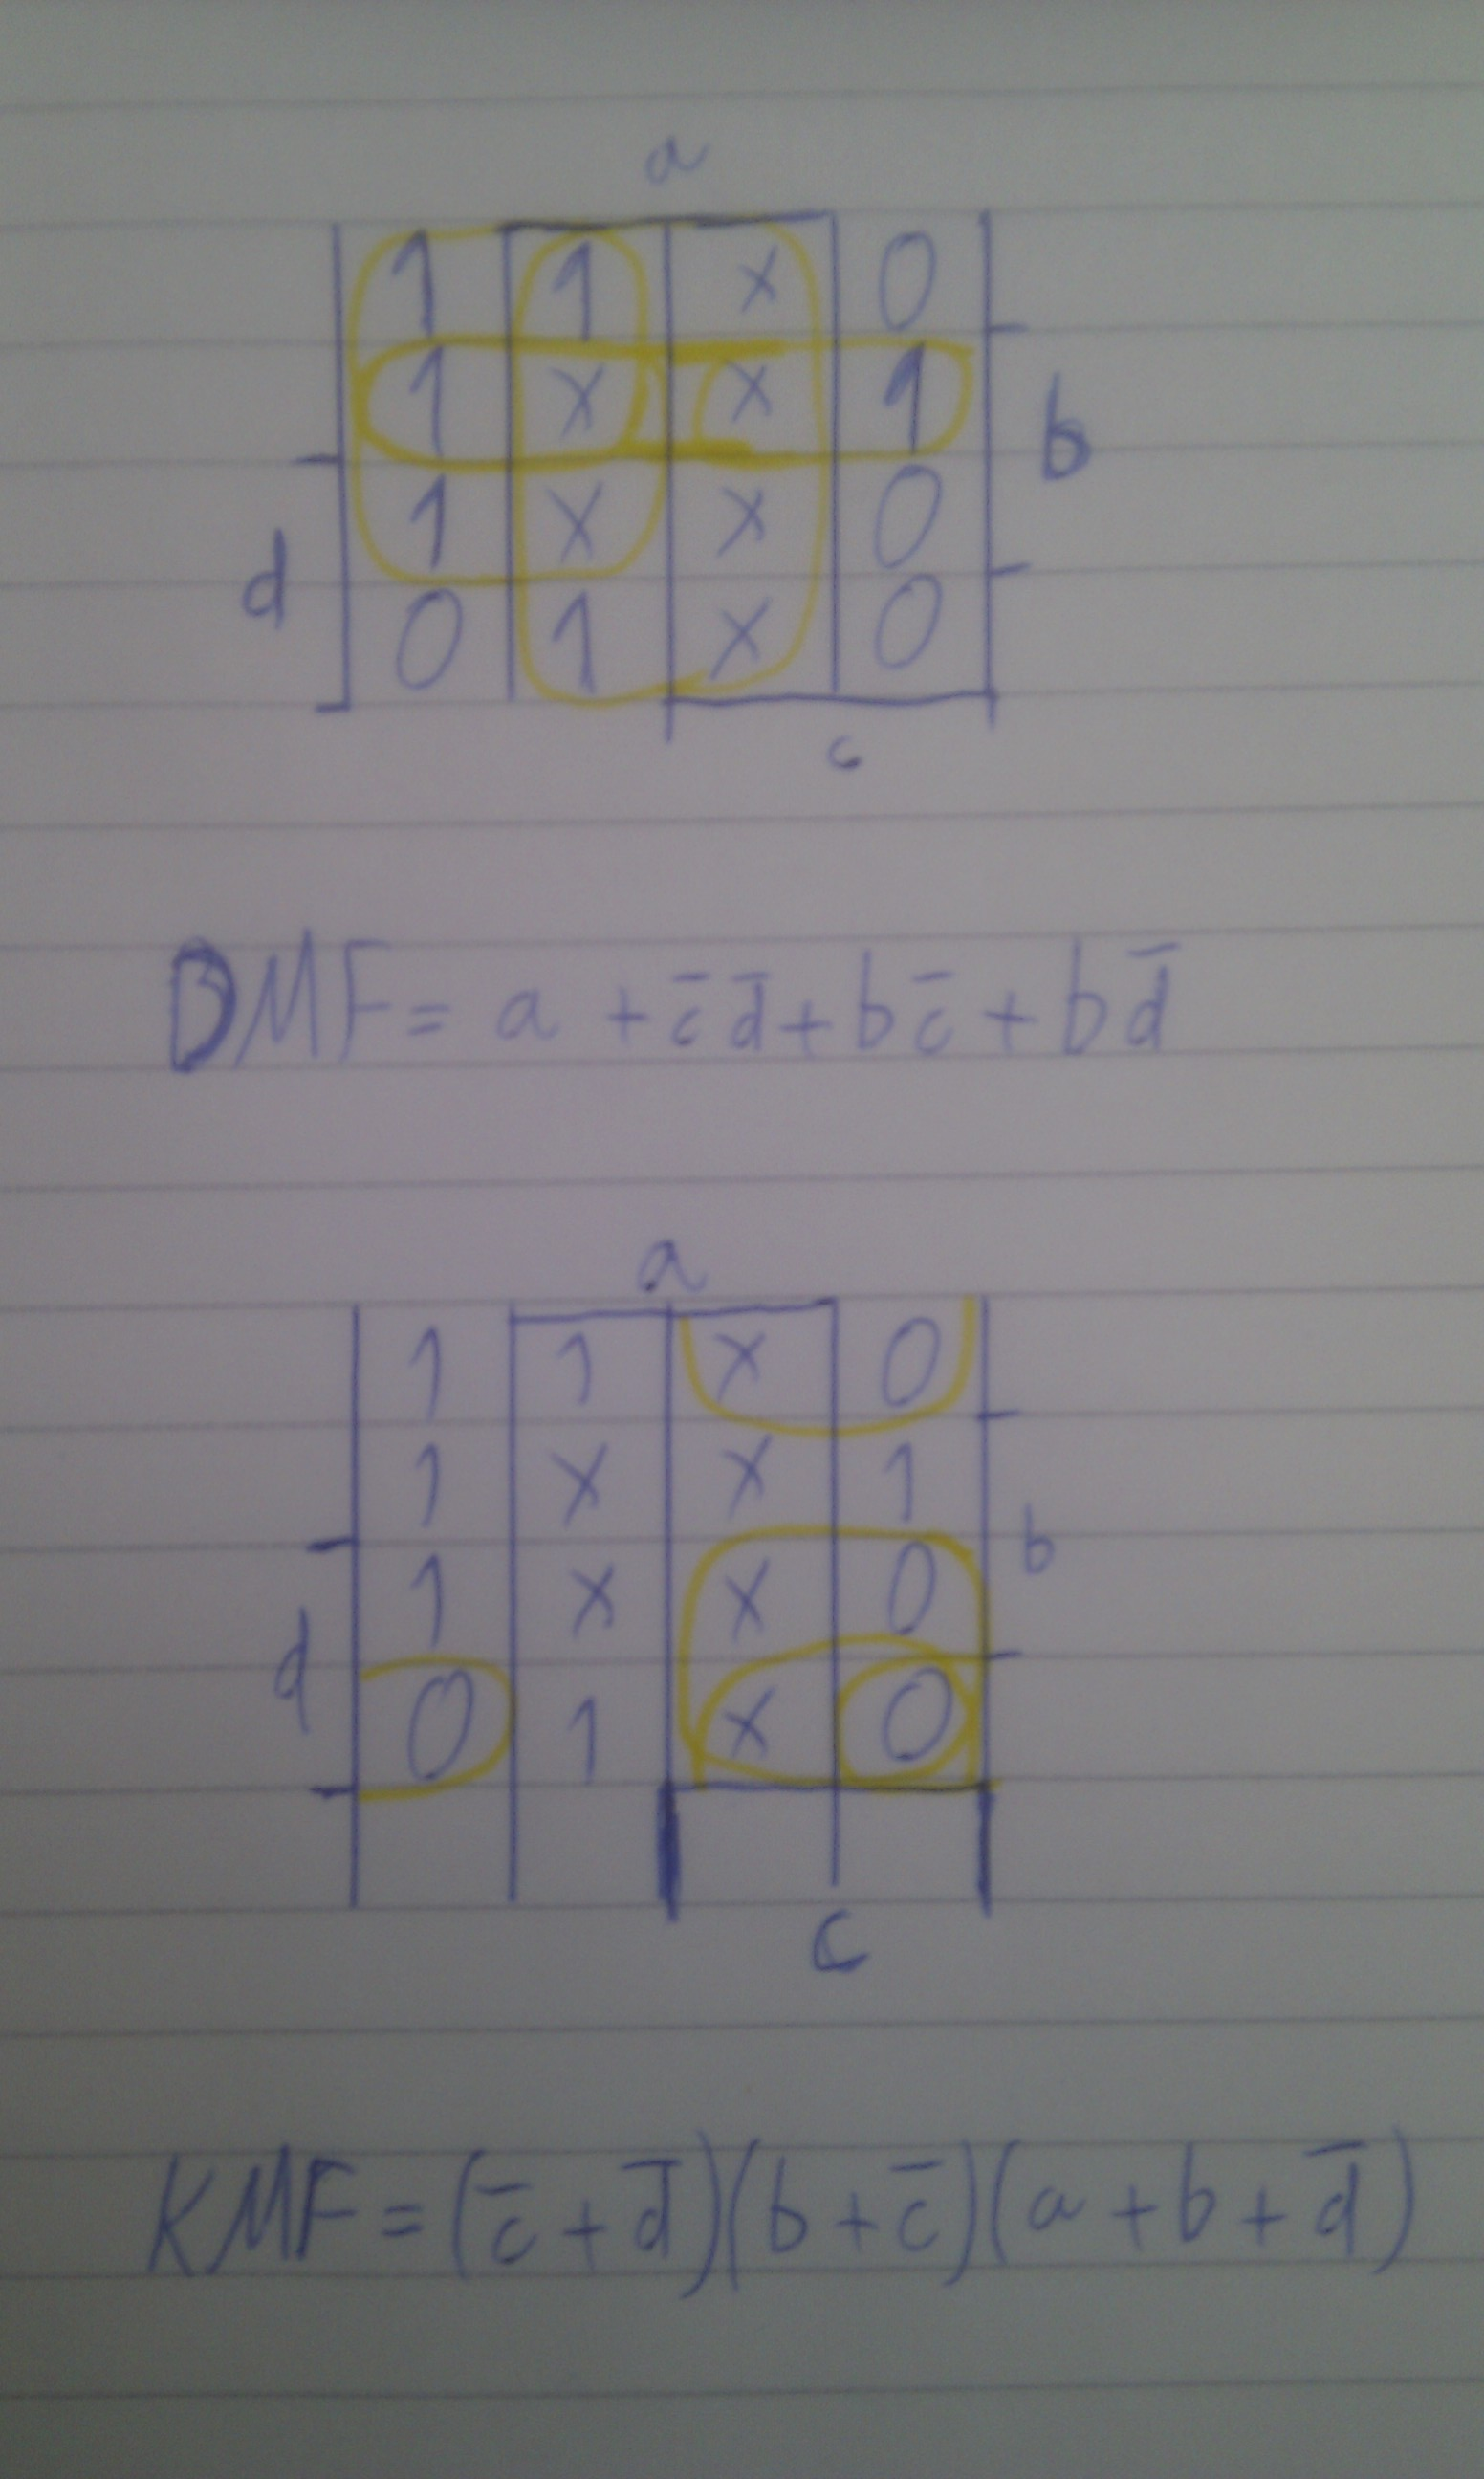
\includegraphics[width=200pt]{11_3}
\end{figure}

\section*{Aufgabe 11.4}

\subsection*{Teil 1}

Da alle 3 Bauteile byteweise operieren und wir einen 8 Bit breiten Datenbus haben, haben alle Chips 8 Datenleitungen.
Um 4M byteweise addressieren zu können, benötigen die DRAM-Chips 22 Adressleitungen,
die Flashspeicher benötigen 20 Adressleitungen und die IO-Chips benötigen 2, um ihre 3 Ausgängen anzusprechen.

\subsection*{Teil 2}

Man braucht einen IO-Chip, auf dessen 3 Ausgängen die untersten 3 Bytes des Addressraums abgebildet werden.
Dazu braucht man noch 3x Flash und 1x DRAM.

\subsection*{Teil 3}
Da unbenutzte Adressen nicht angesprochen werden, lässt sich der Adressraum in 16 Teile unterteilen, die man anhand der 4 höchstwertigen Bits unterscheiden kann.
\begin{figure}[h]
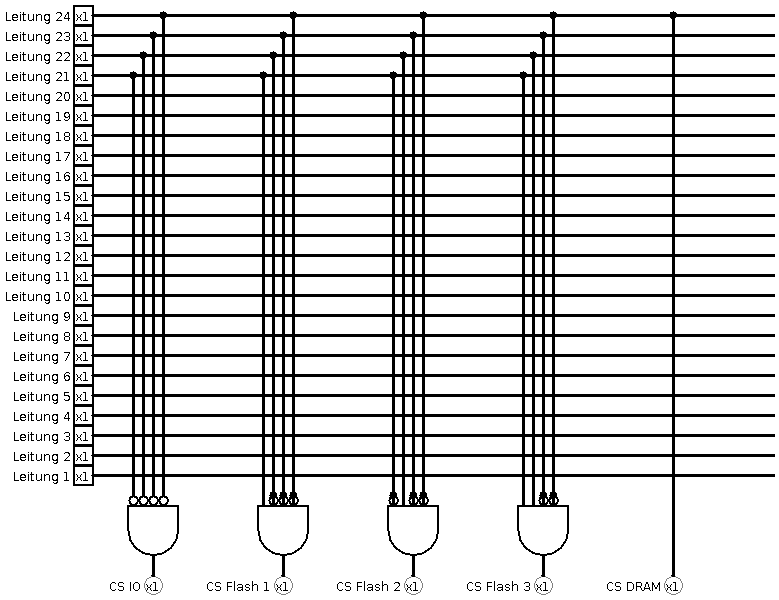
\includegraphics[width=400pt]{11_4_3}
\end{figure}

\subsection*{Teil 4}

An den IO-Chip werden Leitung 1 und 2, an die Flashspeicher Leitung 1-20 und an den DRAM Leitung 1-22 angeschlossen.
Das funktioniert, weil die Adressräume den Chips immer so zugewiesen sind, dass z.B. beim Flashspeicher 3 die obersten 4 Bit den Chip/1-MB-Speicherblock auswählen und die unteren 20 Bit nur innerhalb dieses Blocks adressieren.
Also kann man mit diesen 20 Bit den gesamten Chip adressieren.

\subsection*{Teil 5}

Alle Chips werden an die 8 Datenleitungen angeschlossen.
Das funktioniert, weil immer nur der Chip aktiv ist, der gerade $\overline{CS}$ bekommt.

\end{document}